\chapter{Conclusions and Discussion}
As stated in the introduction, the goal of the project was to use consumer energy time series data to identify clusters of consumption patters and combine the results of which with geographic and demographic data to build a classifier to identify what cluster a consumer belongs to.

When we performed the clustering (on consumption data based on the mean energy consumption per half-hour) on the first chunk of data, we found 3 distinct clusters. These groups can be described as:
    \begin{itemize}
        \item Cluster 1: Low energy consumption and low variance
        \item Cluster 2: High energy consumption, medium variance
        \item Cluster 3: High energy consumption, high variance
    \end{itemize}
    
Each ANON\_ID in the chunk was then assigned to a cluster id. This then enabled us to merge the ANON\_ID and cluster id with the geographic data set. This new data set allowed us to analyse the geographic variables in relation to the cluster id. After pre-processing, the data set could now be passed into a Random Forest model to learn the important features from the geographic data set in order to predict what cluster id a ANON\_ID would belong to.

We saw in section 4.3, results of Random Forest Model, the accuracy of the model was somewhere in the 85-90\% range. However, as cluster group 1 represents ~87\% of the sample size, we could easily create a model with that level of accuracy just by assigning every observation to cluster group 1, which is essentially what this model is doing. The class imbalance as shown in fig.4.2. gives us some insight into why this is happening and also a potential solution. As cluster groups 2 \& 3 have a much lower frequency than cluster group 1, those cluster group observations may be up-sampled in the training set. By learning on a balanced training set it increases the signal of the minor class.


Our RF model, while work in progress, with further investigations could use demographic and geographic data set to predict new observations in geographic data set (new energy consumers/customers) without previous time series data. In order to accomplish the valuable use cases for this, as outlined in the introduction, further work must be done in the areas of time series pre-processing into and class balancing.

\begin{figure}[H]
\centering     
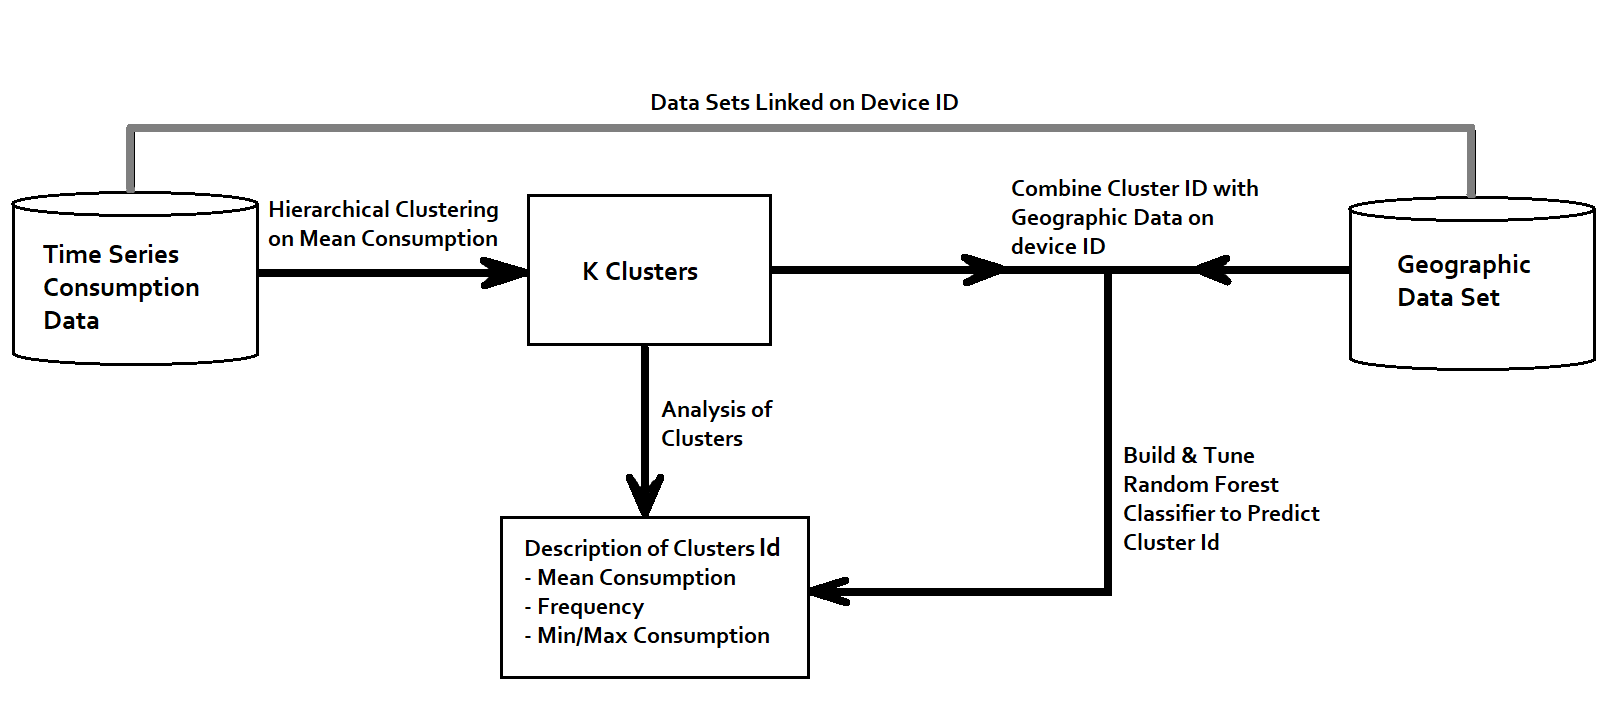
\includegraphics[width=1\textwidth]{Figures/workflow.png}
\caption{Work Flow Carried Out}
\label{fig:Dendrogram}
\end{figure} 

Instead of considering just one chunk of data as per this project, computational performance increases could be made by distributing multiple chunks to different systems and carrying out the same work flow in parallel. This would allow for a greater number of observations to be considered and would greatly enhance the computational efficiency over running this over just one system and by considering a greater number of observations, this would bring the sample mean closer to the true mean and therefore result in a better model.
